\chapter{Two-Dimensional Fermi Liquids: Zero Sound and the Roton Mode}\label{ch08}
% generated by figures/ch08_numbers_tex.py from figures/ch08_numbers.json -- do not edit
\expandafter\def\csname ceight@s0_0p1\endcsname{1.0042}
\expandafter\def\csname ceight@qc_0p1\endcsname{0.008}
\expandafter\def\csname ceight@W_0p1\endcsname{0.0761}
\expandafter\def\csname ceight@frac_0p1\endcsname{0.3056}
\expandafter\def\csname ceight@fracpc_0p1\endcsname{30.6\,\%}
\expandafter\def\csname ceight@amp_0p1\endcsname{0.1667}
\expandafter\def\csname ceight@cont_0p1\endcsname{0.8333}
\expandafter\def\csname ceight@s1_0p1\endcsname{0.7416}
\expandafter\def\csname ceight@s0m1_0p1\endcsname{0.0042}
\expandafter\def\csname ceight@s0_0p5\endcsname{1.0607}
\expandafter\def\csname ceight@qc_0p5\endcsname{0.121}
\expandafter\def\csname ceight@W_0p5\endcsname{0.1768}
\expandafter\def\csname ceight@frac_0p5\endcsname{0.7500}
\expandafter\def\csname ceight@fracpc_0p5\endcsname{75.0\,\%}
\expandafter\def\csname ceight@amp_0p5\endcsname{0.5000}
\expandafter\def\csname ceight@cont_0p5\endcsname{0.5000}
\expandafter\def\csname ceight@s1_0p5\endcsname{0.8660}
\expandafter\def\csname ceight@s0m1_0p5\endcsname{0.0607}
\expandafter\def\csname ceight@s0_1\endcsname{1.1547}
\expandafter\def\csname ceight@qc_1\endcsname{0.309}
\expandafter\def\csname ceight@W_1\endcsname{0.1925}
\expandafter\def\csname ceight@frac_1\endcsname{0.8889}
\expandafter\def\csname ceight@fracpc_1\endcsname{88.9\,\%}
\expandafter\def\csname ceight@amp_1\endcsname{0.6667}
\expandafter\def\csname ceight@cont_1\endcsname{0.3333}
\expandafter\def\csname ceight@s1_1\endcsname{1.0000}
\expandafter\def\csname ceight@s0m1_1\endcsname{0.1547}
\expandafter\def\csname ceight@s0_4\endcsname{1.6667}
\expandafter\def\csname ceight@qc_4\endcsname{1.333}
\expandafter\def\csname ceight@W_4\endcsname{0.1481}
\expandafter\def\csname ceight@frac_4\endcsname{0.9877}
\expandafter\def\csname ceight@fracpc_4\endcsname{98.8\,\%}
\expandafter\def\csname ceight@amp_4\endcsname{0.8889}
\expandafter\def\csname ceight@cont_4\endcsname{0.1111}
\expandafter\def\csname ceight@s1_4\endcsname{1.5811}
\expandafter\def\csname ceight@s0m1_4\endcsname{0.6667}
\expandafter\def\csname ceight@s0_12\endcsname{2.6000}
\expandafter\def\csname ceight@qc_12\endcsname{3.200}
\expandafter\def\csname ceight@W_12\endcsname{0.0960}
\expandafter\def\csname ceight@frac_12\endcsname{0.9984}
\expandafter\def\csname ceight@fracpc_12\endcsname{99.8\,\%}
\expandafter\def\csname ceight@amp_12\endcsname{0.9600}
\expandafter\def\csname ceight@cont_12\endcsname{0.0400}
\expandafter\def\csname ceight@s1_12\endcsname{2.5495}
\expandafter\def\csname ceight@s0m1_12\endcsname{1.6000}
\expandafter\def\csname ceight@s0_40\endcsname{4.5556}
\expandafter\def\csname ceight@qc_40\endcsname{7.111}
\expandafter\def\csname ceight@W_40\endcsname{0.0549}
\expandafter\def\csname ceight@frac_40\endcsname{0.9998}
\expandafter\def\csname ceight@fracpc_40\endcsname{100.0\,\%}
\expandafter\def\csname ceight@amp_40\endcsname{0.9877}
\expandafter\def\csname ceight@cont_40\endcsname{0.0123}
\expandafter\def\csname ceight@s1_40\endcsname{4.5277}
\expandafter\def\csname ceight@s0m1_40\endcsname{3.5556}
\expandafter\def\csname ceight@s3_0p5\endcsname{1.0051}
\expandafter\def\csname ceight@s3_1\endcsname{1.0444}
\expandafter\def\csname ceight@s3_4\endcsname{1.4076}
\expandafter\def\csname ceight@s3_12\endcsname{2.1487}
\expandafter\def\csname ceight@s3m1_0p5\endcsname{0.0051}
\expandafter\def\csname ceight@s3m1_1\endcsname{0.0444}
\expandafter\def\csname ceight@Fstar\endcsname{6.464}
\expandafter\def\csname ceight@Fninety\endcsname{1.081}
\expandafter\def\csname ceight@asymSmall1e3\endcsname{0.9980}
\expandafter\def\csname ceight@asymLarge1e3\endcsname{1.0007}
\expandafter\def\csname ceight@asymLargeThree1e3\endcsname{1.0009}
\expandafter\def\csname ceight@asymThreeSmall\endcsname{1.00000001}
\expandafter\def\csname ceight@partialFracErr\endcsname{\ensuremath{5.7\times10^{-14}}}
\expandafter\def\csname ceight@contErr2\endcsname{\ensuremath{1.0\times10^{-11}}}
\expandafter\def\csname ceight@contRes2\endcsname{\ensuremath{2.0\times10^{-11}}}
\expandafter\def\csname ceight@contSteps2\endcsname{921}
\expandafter\def\csname ceight@contErr3\endcsname{\ensuremath{3.1\times10^{-11}}}
\expandafter\def\csname ceight@contRes3\endcsname{\ensuremath{6.2\times10^{-11}}}
\expandafter\def\csname ceight@contSteps3\endcsname{1269}
\expandafter\def\csname ceight@contPoints\endcsname{81}
\expandafter\def\csname ceight@contRtol\endcsname{\ensuremath{1\times10^{-12}}}
\expandafter\def\csname ceight@sumDev\endcsname{\ensuremath{6.3\times10^{-15}}}
\expandafter\def\csname ceight@sumRel\endcsname{\ensuremath{1.1\times10^{-15}}}
\expandafter\def\csname ceight@sumCont_0p5\endcsname{0.062500}
\expandafter\def\csname ceight@sumPole_0p5\endcsname{0.187500}
\expandafter\def\csname ceight@sumCont_1\endcsname{0.027778}
\expandafter\def\csname ceight@sumPole_1\endcsname{0.222222}
\expandafter\def\csname ceight@sumCont_4\endcsname{0.003086}
\expandafter\def\csname ceight@sumPole_4\endcsname{0.246914}
\expandafter\def\csname ceight@errU_m0p5\endcsname{\ensuremath{4.0\times10^{-9}}}
\expandafter\def\csname ceight@edrift_m0p5\endcsname{\ensuremath{3.2\times10^{-8}}}
\expandafter\def\csname ceight@stepsU_m0p5\endcsname{3\,910}
\expandafter\def\csname ceight@rhsU_m0p5\endcsname{9\,024}
\expandafter\def\csname ceight@wallU_m0p5\endcsname{16.6}
\expandafter\def\csname ceight@errU_0\endcsname{\ensuremath{1.7\times10^{-8}}}
\expandafter\def\csname ceight@edrift_0\endcsname{\ensuremath{1.1\times10^{-7}}}
\expandafter\def\csname ceight@stepsU_0\endcsname{3\,947}
\expandafter\def\csname ceight@rhsU_0\endcsname{9\,179}
\expandafter\def\csname ceight@wallU_0\endcsname{7.1}
\expandafter\def\csname ceight@errU_0p5\endcsname{\ensuremath{6.5\times10^{-8}}}
\expandafter\def\csname ceight@edrift_0p5\endcsname{\ensuremath{1.5\times10^{-7}}}
\expandafter\def\csname ceight@stepsU_0p5\endcsname{4\,133}
\expandafter\def\csname ceight@rhsU_0p5\endcsname{9\,700}
\expandafter\def\csname ceight@wallU_0p5\endcsname{25.9}
\expandafter\def\csname ceight@errU_1\endcsname{\ensuremath{1.2\times10^{-7}}}
\expandafter\def\csname ceight@edrift_1\endcsname{\ensuremath{2.5\times10^{-7}}}
\expandafter\def\csname ceight@stepsU_1\endcsname{4\,370}
\expandafter\def\csname ceight@rhsU_1\endcsname{10\,391}
\expandafter\def\csname ceight@wallU_1\endcsname{69.9}
\expandafter\def\csname ceight@errU_4\endcsname{\ensuremath{3.1\times10^{-7}}}
\expandafter\def\csname ceight@edrift_4\endcsname{\ensuremath{6.5\times10^{-7}}}
\expandafter\def\csname ceight@stepsU_4\endcsname{5\,963}
\expandafter\def\csname ceight@rhsU_4\endcsname{15\,015}
\expandafter\def\csname ceight@wallU_4\endcsname{13.6}
\expandafter\def\csname ceight@errU_12\endcsname{\ensuremath{1.0\times10^{-6}}}
\expandafter\def\csname ceight@edrift_12\endcsname{\ensuremath{2.0\times10^{-6}}}
\expandafter\def\csname ceight@stepsU_12\endcsname{7\,935}
\expandafter\def\csname ceight@rhsU_12\endcsname{20\,720}
\expandafter\def\csname ceight@wallU_12\endcsname{68.9}
\expandafter\def\csname ceight@errK_m0p5\endcsname{\ensuremath{1.4\times10^{-9}}}
\expandafter\def\csname ceight@errK_0p5\endcsname{\ensuremath{2.1\times10^{-8}}}
\expandafter\def\csname ceight@errK_1\endcsname{\ensuremath{3.1\times10^{-8}}}
\expandafter\def\csname ceight@errK_4\endcsname{\ensuremath{9.0\times10^{-8}}}
\expandafter\def\csname ceight@errK_12\endcsname{\ensuremath{1.8\times10^{-7}}}
\expandafter\def\csname ceight@fitW_0p5\endcsname{\ensuremath{1.8\times10^{-10}}}
\expandafter\def\csname ceight@fitA_0p5\endcsname{\ensuremath{7.6\times10^{-8}}}
\expandafter\def\csname ceight@fitW_1\endcsname{\ensuremath{2.4\times10^{-10}}}
\expandafter\def\csname ceight@fitA_1\endcsname{\ensuremath{1.0\times10^{-7}}}
\expandafter\def\csname ceight@fitW_4\endcsname{\ensuremath{2.6\times10^{-10}}}
\expandafter\def\csname ceight@fitA_4\endcsname{\ensuremath{1.7\times10^{-7}}}
\expandafter\def\csname ceight@fitW_12\endcsname{\ensuremath{6.4\times10^{-10}}}
\expandafter\def\csname ceight@fitA_12\endcsname{\ensuremath{5.2\times10^{-7}}}
\expandafter\def\csname ceight@omegaFit4\endcsname{1.666666667}
\expandafter\def\csname ceight@ampFit4\endcsname{0.888889}
\expandafter\def\csname ceight@omegaFit12\endcsname{2.60000000}
\expandafter\def\csname ceight@omegaFit05\endcsname{1.060660172}
\expandafter\def\csname ceight@sZeroHalf\endcsname{1.060660172}
\expandafter\def\csname ceight@expo_m0p5\endcsname{-1.497}
\expandafter\def\csname ceight@expo_0\endcsname{-0.500}
\expandafter\def\csname ceight@expo_1\endcsname{-1.350}
\expandafter\def\csname ceight@expo_4\endcsname{-1.479}
\expandafter\def\csname ceight@tol_bdf_06\endcsname{\ensuremath{5.0\times10^{-7}}}
\expandafter\def\csname ceight@tolsteps_bdf_06\endcsname{3\,488}
\expandafter\def\csname ceight@tol_adams_06\endcsname{\ensuremath{1.1\times10^{1}}}
\expandafter\def\csname ceight@tolsteps_adams_06\endcsname{1\,018}
\expandafter\def\csname ceight@tol_bdf_08\endcsname{\ensuremath{1.7\times10^{-8}}}
\expandafter\def\csname ceight@tolsteps_bdf_08\endcsname{3\,947}
\expandafter\def\csname ceight@tol_adams_08\endcsname{\ensuremath{1.9\times10^{-1}}}
\expandafter\def\csname ceight@tolsteps_adams_08\endcsname{1\,374}
\expandafter\def\csname ceight@tol_bdf_10\endcsname{\ensuremath{1.7\times10^{-9}}}
\expandafter\def\csname ceight@tolsteps_bdf_10\endcsname{5\,828}
\expandafter\def\csname ceight@tol_adams_10\endcsname{\ensuremath{4.0\times10^{-4}}}
\expandafter\def\csname ceight@tolsteps_adams_10\endcsname{2\,585}
\expandafter\def\csname ceight@adamsF4\endcsname{1.77}
\expandafter\def\csname ceight@nNinetySix\endcsname{\ensuremath{4.9\times10^{-8}}}
\expandafter\def\csname ceight@wallNinetySix\endcsname{23}
\expandafter\def\csname ceight@wallSixtyFour\endcsname{13.6}
\expandafter\def\csname ceight@normDrift\endcsname{\ensuremath{1.1\times10^{-7}}}
\expandafter\def\csname ceight@mSqEnd\endcsname{0.0084}
\expandafter\def\csname ceight@growthPred\endcsname{0.577350}
\expandafter\def\csname ceight@growthFit\endcsname{0.577350}
\expandafter\def\csname ceight@growthEdrift\endcsname{\ensuremath{3.2\times10^{-6}}}
\expandafter\def\csname ceight@wallZeroA\endcsname{7.1}
\expandafter\def\csname ceight@wallZeroB\endcsname{12.7}
\expandafter\def\csname ceight@reconF0\endcsname{\ensuremath{7.3\times10^{-8}}}
\expandafter\def\csname ceight@reconF4\endcsname{\ensuremath{3.7\times10^{-5}}}
\expandafter\def\csname ceight@nuMaxFour12\endcsname{3.40}
\expandafter\def\csname ceight@nuMinFour24\endcsname{0.13}
\expandafter\def\csname ceight@mod_stale_bdf_06\endcsname{\ensuremath{2.0\times10^{-6}}}
\expandafter\def\csname ceight@mod_stale_bdf_08\endcsname{failed}
\expandafter\def\csname ceight@mod_stale_bdf_10\endcsname{failed}
\expandafter\def\csname ceight@modB_stale_bdf\endcsname{\ensuremath{5.0\times10^{-7}}}
\expandafter\def\csname ceight@mod_stale_adams_06\endcsname{\ensuremath{1.9\times10^{-4}}}
\expandafter\def\csname ceight@mod_stale_adams_08\endcsname{\ensuremath{1.9\times10^{-5}}}
\expandafter\def\csname ceight@mod_stale_adams_10\endcsname{\ensuremath{1.9\times10^{-6}}}
\expandafter\def\csname ceight@modB_stale_adams\endcsname{\ensuremath{7.2\times10^{-4}}}
\expandafter\def\csname ceight@mod_fresh_bdf_06\endcsname{\ensuremath{1.9\times10^{-7}}}
\expandafter\def\csname ceight@mod_fresh_bdf_08\endcsname{\ensuremath{9.5\times10^{-10}}}
\expandafter\def\csname ceight@mod_fresh_bdf_10\endcsname{\ensuremath{1.4\times10^{-10}}}
\expandafter\def\csname ceight@modB_fresh_bdf\endcsname{\ensuremath{5.0\times10^{-7}}}
\expandafter\def\csname ceight@mod_fresh_adams_06\endcsname{\ensuremath{1.7\times10^{-7}}}
\expandafter\def\csname ceight@mod_fresh_adams_08\endcsname{\ensuremath{1.8\times10^{-9}}}
\expandafter\def\csname ceight@mod_fresh_adams_10\endcsname{\ensuremath{1.7\times10^{-10}}}
\expandafter\def\csname ceight@modB_fresh_adams\endcsname{\ensuremath{2.0\times10^{-8}}}
\expandafter\def\csname ceight@modStaleDate\endcsname{2026-09-26}
\expandafter\def\csname ceight@modFreshCommit\endcsname{5db8041}
\expandafter\def\csname ceight@sweepAdamsBad\endcsname{\ensuremath{3.3\times10^{-3}}}
\expandafter\def\csname ceight@sweepAdamsBadFD\endcsname{\ensuremath{4.7\times10^{-2}}}
\expandafter\def\csname ceight@sweepAdamsGoodMax\endcsname{\ensuremath{1.5\times10^{-7}}}
\expandafter\def\csname ceight@sweepAdamsGoodMin\endcsname{\ensuremath{1.1\times10^{-11}}}
\expandafter\def\csname ceight@sweepBdfMax\endcsname{\ensuremath{1.2\times10^{-6}}}
\expandafter\def\csname ceight@sweepBdfMin\endcsname{\ensuremath{3.3\times10^{-8}}}
\expandafter\def\csname ceight@vmW_0p3\endcsname{1.1598}
\expandafter\def\csname ceight@vmG_0p3\endcsname{0.0126}
\expandafter\def\csname ceight@vmWs_0p3\endcsname{1.1597}
\expandafter\def\csname ceight@vmGs_0p3\endcsname{0.0127}
\expandafter\def\csname ceight@vmRelG_0p3\endcsname{0.78\,\%}
\expandafter\def\csname ceight@vmRelW_0p3\endcsname{0.015\,\%}
\expandafter\def\csname ceight@vmW_0p4\endcsname{1.2851}
\expandafter\def\csname ceight@vmG_0p4\endcsname{0.0661}
\expandafter\def\csname ceight@vmWs_0p4\endcsname{1.2846}
\expandafter\def\csname ceight@vmGs_0p4\endcsname{0.0663}
\expandafter\def\csname ceight@vmRelG_0p4\endcsname{0.28\,\%}
\expandafter\def\csname ceight@vmRelW_0p4\endcsname{0.036\,\%}
\expandafter\def\csname ceight@vmW_0p5\endcsname{1.4157}
\expandafter\def\csname ceight@vmG_0p5\endcsname{0.1534}
\expandafter\def\csname ceight@vmWs_0p5\endcsname{1.4156}
\expandafter\def\csname ceight@vmGs_0p5\endcsname{0.1535}
\expandafter\def\csname ceight@vmRelG_0p5\endcsname{0.09\,\%}
\expandafter\def\csname ceight@vmRelW_0p5\endcsname{0.005\,\%}
\expandafter\def\csname ceight@vmW_0p6\endcsname{1.5457}
\expandafter\def\csname ceight@vmG_0p6\endcsname{0.2641}
\expandafter\def\csname ceight@vmWs_0p6\endcsname{1.5458}
\expandafter\def\csname ceight@vmGs_0p6\endcsname{0.2641}
\expandafter\def\csname ceight@vmRelG_0p6\endcsname{0.01\,\%}
\expandafter\def\csname ceight@vmRelW_0p6\endcsname{0.008\,\%}
\expandafter\def\csname ceight@vmW_0p7\endcsname{1.6739}
\expandafter\def\csname ceight@vmG_0p7\endcsname{0.3924}
\expandafter\def\csname ceight@vmWs_0p7\endcsname{1.6741}
\expandafter\def\csname ceight@vmGs_0p7\endcsname{0.3923}
\expandafter\def\csname ceight@vmRelG_0p7\endcsname{0.02\,\%}
\expandafter\def\csname ceight@vmRelW_0p7\endcsname{0.017\,\%}
\expandafter\def\csname ceight@vmW_0p8\endcsname{1.7999}
\expandafter\def\csname ceight@vmG_0p8\endcsname{0.5346}
\expandafter\def\csname ceight@vmWs_0p8\endcsname{1.8003}
\expandafter\def\csname ceight@vmGs_0p8\endcsname{0.5345}
\expandafter\def\csname ceight@vmRelG_0p8\endcsname{0.02\,\%}
\expandafter\def\csname ceight@vmRelW_0p8\endcsname{0.021\,\%}
\expandafter\def\csname ceight@vmConvMax\endcsname{\ensuremath{1.2\times10^{-6}}}
\expandafter\def\csname ceight@vmCertRe\endcsname{1.415661889}
\expandafter\def\csname ceight@vmCertIm\endcsname{0.153359467}
\expandafter\def\csname ceight@vmProgRe\endcsname{1.415661889}
\expandafter\def\csname ceight@vmProgIm\endcsname{0.153359467}
\expandafter\def\csname ceight@vfW_0p3\endcsname{1.0489}
\expandafter\def\csname ceight@vfWs_0p3\endcsname{1.0492}
\expandafter\def\csname ceight@vfWb_0p3\endcsname{1.0440}
\expandafter\def\csname ceight@vfG_0p3\endcsname{\ensuremath{1.2\times10^{-9}}}
\expandafter\def\csname ceight@vfGs_0p3\endcsname{\ensuremath{2.6\times10^{-6}}}
\expandafter\def\csname ceight@vfRelW_0p3\endcsname{0.037\,\%}
\expandafter\def\csname ceight@vfRes_0p3\endcsname{\ensuremath{1.8\times10^{-3}}}
\expandafter\def\csname ceight@vfRelG_0p3\endcsname{109322.51\,\%}
\expandafter\def\csname ceight@vfW_0p5\endcsname{1.1337}
\expandafter\def\csname ceight@vfWs_0p5\endcsname{1.1339}
\expandafter\def\csname ceight@vfWb_0p5\endcsname{1.1180}
\expandafter\def\csname ceight@vfG_0p5\endcsname{\ensuremath{8.6\times10^{-5}}}
\expandafter\def\csname ceight@vfGs_0p5\endcsname{\ensuremath{5.9\times10^{-5}}}
\expandafter\def\csname ceight@vfRelW_0p5\endcsname{0.022\,\%}
\expandafter\def\csname ceight@vfRes_0p5\endcsname{\ensuremath{3.6\times10^{-3}}}
\expandafter\def\csname ceight@vfRelG_0p5\endcsname{168.49\,\%}
\expandafter\def\csname ceight@vfW_0p8\endcsname{1.3342}
\expandafter\def\csname ceight@vfWs_0p8\endcsname{1.3341}
\expandafter\def\csname ceight@vfWb_0p8\endcsname{1.2806}
\expandafter\def\csname ceight@vfG_0p8\endcsname{\ensuremath{1.1\times10^{-2}}}
\expandafter\def\csname ceight@vfGs_0p8\endcsname{\ensuremath{1.1\times10^{-2}}}
\expandafter\def\csname ceight@vfRelW_0p8\endcsname{0.007\,\%}
\expandafter\def\csname ceight@vfRes_0p8\endcsname{\ensuremath{4.9\times10^{-3}}}
\expandafter\def\csname ceight@vfRelG_0p8\endcsname{0.70\,\%}
\expandafter\def\csname ceight@vfWeakG_03\endcsname{\ensuremath{1.2\times10^{-9}}}
\expandafter\def\csname ceight@vmCertDiff\endcsname{\ensuremath{4.4\times10^{-16}}}
\expandafter\def\csname ceight@fsMax\endcsname{\ensuremath{3.7\times10^{-9}}}
\expandafter\def\csname ceight@fsFloor\endcsname{\ensuremath{1.9\times10^{-10}}}
\expandafter\def\csname ceight@fsRecur\endcsname{536}
\expandafter\def\csname ceight@consMassM\endcsname{\ensuremath{3.3\times10^{-10}}}
\expandafter\def\csname ceight@consEnM\endcsname{\ensuremath{5.1\times10^{-7}}}
\expandafter\def\csname ceight@consEnF\endcsname{\ensuremath{1.6\times10^{-6}}}
\expandafter\def\csname ceight@fermiA\endcsname{0.499998}
\expandafter\def\csname ceight@vmLost03\endcsname{40\,\%}
\expandafter\def\csname ceight@peakFitFermi05\endcsname{\ensuremath{8.3\times10^{-5}}}
\expandafter\def\csname ceight@epsFS\endcsname{0.10}
\expandafter\def\csname ceight@fsumA\endcsname{-0.4996}
\expandafter\def\csname ceight@fsumB\endcsname{-0.4944}
\expandafter\def\csname ceight@ratioNinetySix\endcsname{1.7}
\expandafter\def\csname ceight@leanAxioms\endcsname{propext, Classical.choice, Quot.sound}
\expandafter\def\csname ceight@leanSeconds\endcsname{36.4}
\expandafter\def\csname ceight@stepsN96\endcsname{6\,000}
\expandafter\def\csname ceight@stepsN64\endcsname{5\,963}

\providecommand{\ceightV}[1]{\ifcsname ceight@#1\endcsname\csname ceight@#1\endcsname\else\PackageError{ch08}{Undefined number key #1}{Run figures/ch08_numbers_tex.py}\fi}
\providecommand{\ceightavg}[1]{\left\langle #1\right\rangle}
% looser float parameters for this chapter (a large figure may share a page with a few paragraphs); restored at the end of the chapter
\renewcommand{\topfraction}{0.88}\renewcommand{\textfraction}{0.08}\renewcommand{\floatpagefraction}{0.75}\setcounter{topnumber}{3}

Send neutrons through a sheet of liquid helium-3 that is one atom thick, and ask, for each momentum $\hbar q$ handed to the sheet, how much energy $\hbar\omega$ the neutrons leave behind.
A gas of free fermions answers with a band: the energies of all the ways of lifting one atom out of the Fermi sea into a state above it.
A superfluid of bosons, helium-4, answers with a single thin line, the phonon--roton branch that Landau predicted and that neutrons later traced (\cref{ch05}).
The two-dimensional Fermi liquid studied by Godfrin and his collaborators answers with both, one after the other.
At small $q$ the band is accompanied by a collective density oscillation, of the kind Landau called zero sound, lying just above it; at intermediate $q$ the oscillation runs into the band and is strongly broadened; and at wave vectors larger than twice the Fermi wave vector a well-defined excitation with a roton-like minimum reappears, in a regime where Landau's theory has nothing to say \cite{Godfrin2010,Godfrin2012}.
The third of these gives the chapter its title.

This chapter does not reproduce that measurement, and the reason is part of what it has to teach.
The third regime lies outside anything the three instruments of this book can treat exactly.
The first two do not: they belong to Landau's theory of a Fermi liquid, here collisionless, in two dimensions, with one dimensionless interaction parameter $F$.
For that model the proof assistant can say, once and for all, when an undamped zero-sound wave exists and where it sits; pencil and paper can say how the weight of the neutron spectrum is shared between the wave and the band; and CVODE, integrating the equation of motion in time, can be held against the pencil to $10^{-6}$ or better and made to show how a density wave dies out although nothing is dissipated.
The last section turns to the missing regime, proves the one piece of kinematics that is exact about it, and says where the model stops.

One caution runs through everything below.
The two-dimensional Landau parameters of the film measured by Godfrin and his collaborators are \emph{not known to this book}: no open numerical table of them was found, and the programme's two literature searches came back empty.
The parameter $F$ is therefore left free, every curve is a function of $F$, and no number here is a prediction for the film.

%% ====================================================================================================================
\section{What the neutrons saw}\label{ch08:sec-measure}

\begin{godfrinbox}{What was measured}
\textbf{Experiment.} Inelastic neutron scattering at the Institut Laue--Langevin, Grenoble, on two-dimensional liquid $^3$He: a monolayer of $^3$He adsorbed on graphite preplated with a monolayer of solid $^4$He \cite{Godfrin2010,Godfrin2012}.
The 2012 paper is H.~Godfrin, M.~Meschke, H.-J.~Lauter, A.~Sultan, H.~M.~B\"ohm, E.~Krotscheck and M.~Panholzer, \emph{Nature} \textbf{483}, 576--579 (published 29 March 2012); an earlier paper on the same measurements is \cite{Godfrin2010}.\par\vspace{2pt}
\textbf{What the abstracts report.}
(i) The particle--hole excitations of the two-dimensional Fermi liquid and, above the particle--hole band, the zero-sound mode; at low wave vectors this mode lies very close to the band, contrary to bulk $^3$He.
(ii) At intermediate wave vectors the collective mode enters the band, where it is strongly broadened by Landau damping.
(iii) At wave vectors larger than twice the Fermi wave vector the collective density mode reappears as a well-defined, roton-like excitation, with a dispersion relation ``quite similar to that of superfluid $^4$He''.
The dynamics of Fermi liquids at high wave vectors had been believed ``essentially incoherent''; the authors find ``unexpected collective behaviour'' beyond the scope of Landau's theory and interpret the spectra with a dynamic many-body theory.
The authors' copy of the 2012 paper (open archive HAL, hal-00920422) names the instrument: the time-of-flight spectrometer IN6 of the ILL.\par\vspace{2pt}
\textbf{What this chapter does not have:} any number from those spectra (energies, wave vectors, densities) and the film's Landau parameters. Where it says what a measurement decided, it quotes the abstracts and goes no further.
\end{godfrinbox}

Why was this hard, and what did it decide?
A single adsorbed layer holds very little matter compared with a bulk sample, so the scattering signal is small, and a collective mode has to be recognised on top of a particle--hole band that is broad.
The three regimes of the box are three questions put to the same spectrum: where is the collective mode while Landau's theory applies, what happens when it meets the band, and does anything survive beyond.
The expected answer to the third was ``no'': a mode that has entered the band is damped, and nothing in the theory brings it back.
The measurement decided that the answer is ``yes'' for a two-dimensional Fermi liquid, which is a statement about nature that no model in this chapter could have supplied.

It helps to hold the $(q,\omega)$ plane in mind.
Lift one fermion out of a Fermi sea of radius $k_F$ and give it momentum $\hbar q$: the energies it can absorb fill a band, bounded above by $\hbar v_Fq+\hbar^2q^2/2m$ and, for $q<2k_F$, below by zero.
A density wave can be a sharp excitation only if its dispersion lies outside the band; inside, it can decay into pairs and is broadened.
At small $q$ Landau's theory says where such a wave sits, and at larger $q$ the line it draws enters the band.
The abstract of the 2012 paper names the wave vector $2k_F$, at which the band itself changes character because its lower edge lifts off $\omega=0$; \cref{ch08:sec-window} proves that and draws the plane in \cref{ch08:fig-window}.

%% ====================================================================================================================
\section{A Fermi liquid with one number}\label{ch08:sec-model}

Landau's picture keeps what survives of the free Fermi gas \cite{Landau1957,BaymPethick1991}.
The low-lying states are quasi-particles with momentum near the Fermi circle $|\mathbf p|=p_F$; the only state variable of the linear theory is how far the Fermi circle has been pushed outwards (in energy units) in the direction $\theta$, at the place $x$ and the time $t$, a function $\nu(\theta;x,t)$.
A density wave is a Fermi circle that breathes in a travelling pattern.
The quasi-particles interact through the Landau function, whose dimensionless form is $F(\theta-\theta')=N(0)f(\theta-\theta')$, with $N(0)$ the density of states at the Fermi level.
We keep one number from it, the isotropic spin-symmetric part $F\equiv F_0^s$, and set the rest to zero.
That is a model with four honest costs: with $F_1^s=0$ the effective mass equals the bare mass, which is not a good description of helium; the spin-antisymmetric channel is dropped; there are no collisions, so the theory describes $\omega\tau\gg1$, the regime in which zero sound exists, at zero temperature; and the curvature of the quasi-particle spectrum is dropped, so everything is a statement about $q\ll k_F$ and $\hbar\omega\ll E_F$.

For a perturbation along $x$ the linearised, collisionless Landau kinetic equation reads
\begin{equation}\label{ch08:eq-kinetic}
\partial_t\nu+v_F\cos\theta\;\partial_x\bigl[\nu+F\,\ceightavg{\nu}\bigr]=0,\qquad \ceightavg{\nu}=\frac1{2\pi}\int_0^{2\pi}\nu\,\dd\theta,\qquad \delta n=N(0)\,\ceightavg{\nu}.
\end{equation}
The first term is free streaming: the part of the Fermi circle at angle $\theta$ is carried along $x$ with velocity $v_F\cos\theta$.
The second is the mean-field push, $F$ times the density deviation, the same for every $\theta$.
Free streaming plus a force from the mean field is also the structure of the Vlasov equation of a plasma, a likeness that \cref{ch08:sec-vlasov} uses and puts to a test.

A plane wave $\nu\propto\ee^{\ii(qx-\omega t)}$, with $s=\omega/(v_Fq)$, turns \eqref{ch08:eq-kinetic} into $(s-\cos\theta)\,\nu=F\cos\theta\,\ceightavg{\nu}$; dividing by $s-\cos\theta$ and averaging over the angle leaves the dispersion relation
\begin{equation}\label{ch08:eq-disp}
1+F\,\Omega(s)=0,\qquad \Omega(s)=\Bigl\langle\frac{\cos\theta}{\cos\theta-s}\Bigr\rangle=1-s\Bigl\langle\frac1{s-\cos\theta}\Bigr\rangle ,
\end{equation}
where $\Omega$ is the angular average of the response of free quasi-particles.
On a circle the average is algebraic; on a sphere it is a logarithm:
\begin{align}
\Omega_{2\mathrm D}(s)&=1-\frac{s}{\sqrt{s^2-1}}\quad(s>1),\qquad \Omega_{2\mathrm D}(s)=1+\ii\,\frac{s}{\sqrt{1-s^2}}\quad(0<s<1),\label{ch08:eq-Omega}\\
\Omega_{3\mathrm D}(s)&=1-\frac s2\ln\frac{s+1}{s-1}\quad(s>1).\nonumber
\end{align}
For $s>1$ the wave is faster than every quasi-particle and $\Omega$ is real.
For $0<s<1$ some quasi-particles move along $x$ at exactly the phase velocity, $v_F\cos\theta=\omega/q$; they surf the wave and exchange energy with it, and $\Omega$ acquires an imaginary part (its sign fixed by $\omega\to\omega+\ii0$).
That is Landau damping, and the strip $0<\omega<v_Fq$ is the particle--hole continuum.

An undamped wave needs a real root with $s>1$.
In both dimensions $\Omega(s)<0$ for $s>1$, so $\Omega(s)=-1/F$ can be solved only if $F>0$: a repulsive interaction pushes the wave out of the continuum; an attractive one leaves nothing sharp.
In two dimensions the root can be written down; squaring \eqref{ch08:eq-disp} and using $(1+F)^2-F^2=1+2F$ gives
\begin{equation}\label{ch08:eq-root}
s_0=\frac{1+F}{\sqrt{1+2F}},\qquad s_0^2-1=\frac{F^2}{1+2F}\qquad(F>0),
\end{equation}
and $s_0^2=\tfrac F2+\tfrac34+\tfrac1{4(1+2F)}$ shows the strong-coupling limit at a glance.
Weak coupling: $s_0-1\simeq F^2/2$ (the ratio is $\ceightV{asymSmall1e3}$ at $F=10^{-3}$), so the wave leaves the edge of the continuum only quadratically in $F$.
Strong coupling: $s_0\to\sqrt{F/2}$.
In three dimensions the same limits are $s-1\simeq2\,\ee^{-2-2/F}$ and $s\to\sqrt{F/3}$: the sphere lets the wave hug the edge exponentially closely, the circle only quadratically (\cref{ch08:tab-roots}).
Within the model, ``very close to the particle-hole band'', in the words of the 2010 abstract, means a small $F$: $s_0-1$ is $\ceightV{s0m1_0p5}$ at $F=\tfrac12$ and $\ceightV{s0m1_12}$ at $F=12$.
That is the model's way of speaking about the abstract's sentence; it does not determine the film's $F$.

Two further facts about \eqref{ch08:eq-disp}.
At strong coupling the zero-sound speed approaches the hydrodynamic first-sound speed $v_F\sqrt{(1+F)/2}$ (from $c_1^2=(n/m)\,\partial\mu/\partial n$, $\partial\mu/\partial n=(1+F)/N(0)$); the model has no collisions and does not compute the crossover, the two formulas merely meet.
And in the static limit $\Omega(0)=1$, so the compressibility is $1/(1+F)$ times its free value and $F>-1$ is the Pomeranchuk bound, on either side of which \cref{ch08:sec-dephasing} sees the model change its behaviour.

\begin{table}[tp]
\centering\small
\caption{\textbf{The model's numbers} (closed forms). $s_0$: the two-dimensional zero-sound root (Lean: \Lthm{ZeroSound}{zero_sound_2d_iff}); $s$: the three-dimensional root of $g_3(s)=1/F$, for contrast; $q_c/k_F=2(s_0-1)$: where the line $\omega=s_0v_Fq$ meets the free-gas band edge $v_Fq+\hbar q^2/2m$; $W$, ``pole share'': the weight of the line in the structure factor and its share of the $f$-sum rule (\cref{ch08:sec-S}; exactly $\frac89$, $\frac{80}{81}$, $\frac{624}{625}$ at $F=1,4,12$); ``amplitude'': the undamped part of the density after a released wave (\cref{ch08:sec-cvode}).}\label{ch08:tab-roots}
\begin{tabular}{@{}r@{\quad}c@{\quad}c@{\quad}c@{\quad}c@{\quad}c@{\quad}c@{}}
\toprule
$F$ & $s_0$ (2D) & $s$ (3D) & $q_c/k_F$ & $W$ & pole share & amplitude\\
\midrule
$\tfrac12$ & \ceightV{s0_0p5} & \ceightV{s3_0p5} & \ceightV{qc_0p5} & \ceightV{W_0p5} & \ceightV{frac_0p5} & \ceightV{amp_0p5}\\
$1$ & \ceightV{s0_1} & \ceightV{s3_1} & \ceightV{qc_1} & \ceightV{W_1} & \ceightV{frac_1} & \ceightV{amp_1}\\
$4$ & \ceightV{s0_4} & \ceightV{s3_4} & \ceightV{qc_4} & \ceightV{W_4} & \ceightV{frac_4} & \ceightV{amp_4}\\
$12$ & \ceightV{s0_12} & \ceightV{s3_12} & \ceightV{qc_12} & \ceightV{W_12} & \ceightV{frac_12} & \ceightV{amp_12}\\
\bottomrule
\end{tabular}
\end{table}

%% ====================================================================================================================
\section{What Lean proves}\label{ch08:sec-lean}

The library module \texttt{ZeroSound} states the existence criterion in both dimensions.
Its header says what it is and what it is not: textbook physics \cite{BaymPethick1991}, machine-checked, with the two-dimensional case included because the measurement of \cref{ch08:sec-measure} is on a film, where the logarithm of three dimensions does not apply.

\begin{leanbox}{ZeroSound}
\begin{lstlisting}[style=lean]
theorem zero_sound_2d_iff (F : ℝ) :
    (∃ s, 1 < s ∧ 1 + F * (1 - s / √(s ^ 2 - 1)) = 0) ↔ 0 < F

-- (proof abridged) for F > 0 the root is (1 + F) / √(1 + 2 * F); key step:
--   have e : ((1 + F) / √(1 + 2 * F)) ^ 2 - 1 = (F / √(1 + 2 * F)) ^ 2 := by
--     rw [div_pow, div_pow, hq2]; field_simp; ring
\end{lstlisting}
\end{leanbox}

In words: an undamped two-dimensional zero-sound wave exists \emph{if and only if} $F>0$.
If a root $s>1$ exists then $s>\sqrt{s^2-1}$, so $\Omega(s)<0$, and $0=1+F\,\Omega(s)$ forces $F>0$.
If $F>0$, the displayed identity gives $\sqrt{s_0^2-1}=F/\sqrt{1+2F}$, hence $s_0/\sqrt{s_0^2-1}=(1+F)/F$ and $1+F\bigl(1-(1+F)/F\bigr)=0$.
That a helium film obeys the equation is physics, and whether its $F$ is positive is a question for the film.

In three dimensions there is no closed form, so the root is pinned instead.

\begin{leanbox}{ZeroSound}
\begin{lstlisting}[style=lean]
noncomputable def g3 (s : ℝ) : ℝ := s / 2 * log ((s + 1) / (s - 1)) - 1

theorem zero_sound_iff (F : ℝ) : (∃ s, 1 < s ∧ g3 s = 1 / F) ↔ 0 < F
\end{lstlisting}
\end{leanbox}

For $c=1/F>0$ the function $g_3$ is continuous on $(1,\infty)$ (\Lthm{ZeroSound}{continuousOn_g3}) and obeys $g_3(s)\ge\frac12\ln\frac2{s-1}-1$ (\Lthm{ZeroSound}{g3_ge}) and $g_3(s)\le1/(s-1)$ (\Lthm{ZeroSound}{g3_le}); at $s=1+2\ee^{-2(c+2)}$ the first bound gives $g_3\ge c$, at $s=1+2/c$ the second gives $g_3\le c/2$, and the intermediate value theorem delivers a root between.
The module says what it does not prove: uniqueness of the three-dimensional root (that needs strict monotonicity of $g_3$), anything about $F_1^s$ or finite temperature, and the damped branch $s<1$.

Uniqueness \emph{is} easy in two dimensions, and the book adds it in a new module, \texttt{Ch08\_ZeroSound2D}, written for this chapter and compiled with the pinned toolchain, with no \texttt{sorry} (axioms in \cref{ch08:honest}); everything in it is elementary.

\begin{leanbox}{Ch08\_ZeroSound2D (new in this book)}
\begin{lstlisting}[style=lean]
noncomputable def omega2 (s : ℝ) : ℝ := 1 - s / √(s ^ 2 - 1)

noncomputable def s0 (F : ℝ) : ℝ := (1 + F) / √(1 + 2 * F)

theorem zero_sound_2d_unique {F s : ℝ} (hs : 1 < s)
    (h : 1 + F * omega2 s = 0) :
    0 < F ∧ s = s0 F
\end{lstlisting}
\end{leanbox}

Together with \Lthm{ZeroSound}{zero_sound_2d_iff} this says: for $F>0$ there is exactly one undamped zero-sound root, namely $s_0$, and for $F\le0$ there is none.
The proof squares the equation: $Fs=(1+F)\sqrt{s^2-1}$ gives $s^2(1+2F)=(1+F)^2$, and $s$ is positive.
(The statement \Lthm{ZeroSound2D}{zero_sound_2d_unique} lives in the new file; the library is unchanged.)

A theorem about the root invites a check of the number.
The root can be \emph{followed} instead of solved: along $u=\ln F$ the variable $w=\ln(s-1)$ obeys the differential equation obtained by differentiating $1+F\Omega(s)=0$,
\begin{equation}\label{ch08:eq-davidenko}
\frac{\dd w}{\dd u}=\frac{s+1}{s+\sqrt{s^2-1}}\quad(\text{2D}),\qquad
\frac{\dd w}{\dd u}=-\frac{g_3(s)}{(s-1)\,g_3'(s)}\quad(\text{3D}).
\end{equation}
CVODE (the Rust crate \texttt{cvode} of rusty-SUNDIALS, BDF, relative tolerance $\ceightV{contRtol}$) integrates \eqref{ch08:eq-davidenko} from $F=0.05$ to $F=1000$ and returns $\ceightV{contPoints}$ points.
Against the Lean closed form the largest relative error in $s$ is $\ceightV{contErr2}$ in two dimensions; against a 40-digit mpmath root it is $\ceightV{contErr3}$ in three; the original equations are satisfied to $\ceightV{contRes2}$ and $\ceightV{contRes3}$ (open circles in \cref{ch08:fig-zerosound}a, which also shows the circle against the sphere).
This checks the solver against the theorem; the theorem needs no checking.

%% ====================================================================================================================
\section{The structure factor, the pole and the sum rule}\label{ch08:sec-S}

A neutron does not see $\nu$; it sees the dynamic structure factor $S(q,\omega)$.
In the model the density response is $\chi=-N(0)\,\Omega/(1+F\Omega)$, and at zero temperature $S=-\pi^{-1}\operatorname{Im}\chi$ for $\omega>0$; write $S(q,\omega)=N(0)\,\hat S(s)$ (the neutron-scattering constants are dropped).
Inside the continuum $\operatorname{Im}\Omega=s/\sqrt{1-s^2}$ and $|1+F\Omega|^2=\bigl[(1+F)^2-(1+2F)s^2\bigr]/(1-s^2)$, so
\begin{equation}\label{ch08:eq-S}
\hat S(s)=\frac{\operatorname{Im}\Omega}{\pi|1+F\Omega|^2}=\frac{s\sqrt{1-s^2}}{\pi[(1+F)^2-(1+2F)s^2]}=\frac{s\sqrt{1-s^2}}{\pi(1+2F)(s_0^2-s^2)},\quad 0<s<1.
\end{equation}
(The closed form agrees with the definition to $\ceightV{sumRel}$ on a grid of $s$ and $F$.)
For $F>0$ the denominator vanishes at $s_0$, just outside the interval, and the continuum is joined by a $\delta$-function: near $s_0$ one has $1+F\Omega\simeq F\,\Omega'(s_0)(s-s_0)$ with $\Omega'(s)=(s^2-1)^{-3/2}$, so the line has the weight
\begin{equation}\label{ch08:eq-W}
W=\frac1{F^2\,\Omega'(s_0)}=\frac{(s_0^2-1)^{3/2}}{F^2}=\frac{F}{(1+2F)^{3/2}} .
\end{equation}

\begin{figure}[tp]
\centering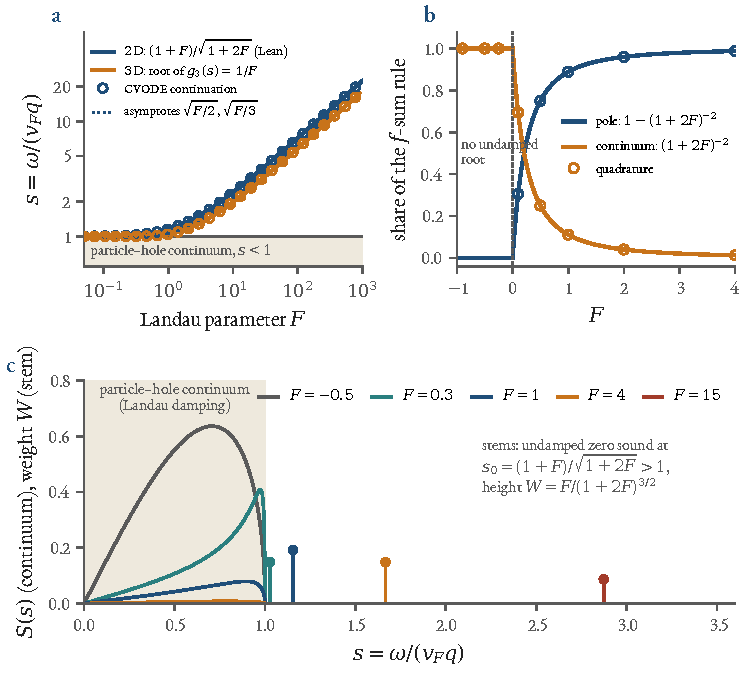
\includegraphics[width=\linewidth]{figures/ch08_zerosound.pdf}
\caption[The zero-sound root and what it carries]{\textbf{The zero-sound root and what it carries.}
\textbf{a}, the root $s(F)$: two dimensions (blue, the Lean closed form), three dimensions (orange, root of $g_3(s)=1/F$); open circles, CVODE continuation of \eqref{ch08:eq-davidenko} ($\ceightV{contPoints}$ points, relative tolerance $\ceightV{contRtol}$); dotted, the asymptotes $\sqrt{F/2}$ and $\sqrt{F/3}$; shaded, the particle--hole continuum $s<1$.
\textbf{b}, shares of the first moment $\int s\hat S\,\dd s=\frac14$: the pole carries $1-(1+2F)^{-2}$ (blue; Lean: \Lthm{ZeroSound2D}{pole_fraction}), the continuum the rest (orange); open circles, quadrature of \eqref{ch08:eq-S}. For $F\le0$ there is no pole.
\textbf{c}, the structure factor \eqref{ch08:eq-S} for five values of $F$ (a curve and its stem have one colour); a stem at $s_0$ has height $W$ of \eqref{ch08:eq-W} and stands for a $\delta$-function.
Script: \texttt{figures/ch08\_zerosound.py}.}\label{ch08:fig-zerosound}
\end{figure}

How much of the spectrum does the line carry?
There is an exact answer.
The function $G(s)=\Omega/(1+F\Omega)$ is analytic in the upper half plane for $F>-1$, and at large $|s|$ one has $\Omega\simeq-1/(2s^2)$, hence $G\simeq-1/(2s^2)$.
Its Hilbert-transform representation $G(s)=\pi^{-1}\!\int\operatorname{Im}G(s')\,(s'-s)^{-1}\dd s'$, with $\operatorname{Im}G$ odd and equal to $\pi\hat S$ for $s>0$, gives $G\simeq-2s^{-2}\int_0^\infty s'\hat S(s')\,\dd s'$, and comparing the two,
\begin{equation}\label{ch08:eq-fsum}
\int_0^\infty s\,\hat S(s)\,\dd s=\frac14\qquad(F>-1),
\end{equation}
which is the $f$-sum rule $\int\omega S\,\dd\omega=nq^2/2m$ of the model (in two dimensions $n=N(0)E_F$ and $E_F=\frac12mv_F^2$).
It holds for every $F$, so a line that exists takes its weight from the band.
The pole contributes $s_0W=F(1+F)/(1+2F)^2$, and since $4F(1+F)=(1+2F)^2-1$ its share is
\begin{equation}\label{ch08:eq-frac}
\frac{s_0W}{1/4}=1-\frac1{(1+2F)^2}\qquad(F>0).
\end{equation}
The identities behind \eqref{ch08:eq-W} and \eqref{ch08:eq-frac} are the new Lean theorems below.
What Lean does \emph{not} prove is that $W$ is the strength of a $\delta$-function in $S$, or that the first moment is $\frac14$: those are the residue theorem and the $f$-sum rule, which the module does not contain.
They are checked numerically: the continuum quadrature plus the pole gives $\frac14$ to $\ceightV{sumDev}$ at eight values of $F$ between $-0.9$ and $15$, and the continuum alone gives $\frac14(1+2F)^{-2}$ for $F>0$ and exactly $\frac14$ for $F\le0$.

\begin{leanbox}{Ch08\_ZeroSound2D (new in this book)}
\begin{lstlisting}[style=lean]
theorem pole_fraction {F : ℝ} (hF : 0 < F) :
    4 * s0 F * (1 / (F ^ 2 * deriv omega2 (s0 F)))
      = 1 - 1 / (1 + 2 * F) ^ 2
\end{lstlisting}
\end{leanbox}

This is \eqref{ch08:eq-frac}, with the residue written $1/(F^2\,\Omega'(s_0))$.
Two further theorems of the new file carry the pieces: \Lthm{ZeroSound2D}{omega2_hasDerivAt} proves $\Omega'(s)=(s^2-1)^{-3/2}$ as a derivative of the function \texttt{omega2}, and \Lthm{ZeroSound2D}{pole_weight} turns that into \eqref{ch08:eq-W}.
The proof of \Lthm{ZeroSound2D}{pole_fraction} is then algebra: the two square roots collapse because $s_0^2-1=F^2/(1+2F)$ (\Lthm{ZeroSound2D}{s0_sq_sub_one}).

Read as physics, \cref{ch08:fig-zerosound}b says that a weak repulsion ($F\to0^+$) gives the line almost no weight, about $4F$ of the sum rule, and leaves it hugging the band, while a strong one pushes it out and gives it almost everything: at $F=4$ the line carries $80/81$.
Whether that says anything about the film the model cannot tell.

%% ====================================================================================================================
\section{Integrating the kinetic equation with CVODE}\label{ch08:sec-cvode}

Equation \eqref{ch08:eq-kinetic} goes onto a computer almost verbatim.
Take units $v_Fq=1$.
For the initial states used below $\nu$ is even in $\theta$, so only $\theta\in(0,\pi)$ is needed, with $N$ midpoint nodes $\theta_j=(j+\tfrac12)\pi/N$ and $\ceightavg{\cdot}\to\frac1N\sum_j$ (a smooth periodic integrand integrated this way is exponentially accurate for times up to order $N$).
With $c_j=\cos\theta_j$ and the real and imaginary parts of $\nu_j$ as unknowns, the system $\dot\nu_j=-\ii c_j(\nu_j+F\ceightavg{\nu})$ is linear with a constant matrix, which is also its Jacobian and is handed to CVODE as such.

\begin{rustbox}{CVODE on the Landau kinetic equation}
Excerpts of the right-hand side and the driver, as run (crate \texttt{cvode} 6.4.0, rusty-SUNDIALS commit \texttt{5db8041}; \texttt{book/rust/ch08\_kinetic}); the closure \texttt{jac} fills the $2N\times2N$ matrix $\left(\begin{smallmatrix}0&A\\-A&0\end{smallmatrix}\right)$, $A_{ij}=c_i\delta_{ij}+c_iF/N$.
\begin{lstlisting}[style=rust]
let rhs = move |_t: f64, y: &[f64], yd: &mut [f64]| -> Result<(), String> {
    let mr = y[..n].iter().sum::<f64>() / nf;
    let mi = y[n..].iter().sum::<f64>() / nf;
    for j in 0..n {
        yd[j] = c_rhs[j] * (y[n + j] + f * mi);
        yd[n + j] = -c_rhs[j] * (y[j] + f * mr);
    }
    Ok(())
};
...
let builder = Cvode::builder(method).rtol(rtol).atol(atol)
    .max_steps(5_000_000);
let builder = if std::env::var("CH08_NOJAC").is_ok() { builder }
    else { builder.jacobian(jac) };
let mut cv = builder.build(rhs, 0.0, SerialVector::from_slice(&y0))
    .expect("build");
...
let (t, y) = cv.solve(tout, Task::Normal)
    .unwrap_or_else(|e| panic!("solve to {tout}: {e:?}"));
\end{lstlisting}
One output ($F=4$, $N=64$, $0\le t\le60$, the density mode $m=\ceightavg\nu$ recorded every $0.1$; the line is the driver's own, copied from \texttt{figures/ch08\_statsline.txt}):
\lstinputlisting[style=plainmono]{figures/ch08_statsline.txt}
Shared eight-core machine, load average 12--35 while these runs were made: wall times are not benchmarks (the same $F=0$ problem took $\ceightV{wallZeroA}$~s and $\ceightV{wallZeroB}$~s in two runs of one batch).
\end{rustbox}

There are exact answers to compare with.
For $F=0$ the nodes decouple and, for the initial state $\nu\equiv1$ (a density wave suddenly released), $m(t)=\ceightavg{\ee^{-\ii t\cos\theta}}=J_0(t)$.
For $F=-\tfrac12$ the Laplace transform of the density is $2/(p+\sqrt{p^2+1})$, whose inverse is $2J_1(t)/t$.
For any $F$ the Laplace transform of $m$ is $\hat m(p)=(p^2+1)^{-1/2}\big/\bigl[1+F\bigl(1-p/\sqrt{p^2+1}\bigr)\bigr]$, which is $\Omega$ continued to imaginary frequency; its singularities are, for $F>0$, the poles $p=\pm\ii s_0$ (residue $F/(1+2F)$ each) and, for every $F$, the cut $|\operatorname{Im}p|<1$ of the square root.
Inverting,
\begin{equation}\label{ch08:eq-uniform}
m(t)=\frac{2F}{1+2F}\cos(s_0t)\;+\;\frac2\pi\int_0^1\frac{(1+F)\sqrt{1-y^2}}{(1+F)^2-(1+2F)y^2}\cos(yt)\,\dd y\qquad(F>0),
\end{equation}
and the same integral alone for $F\le0$; at $t=0$ the two parts are $2F/(1+2F)$ and $1/(1+2F)$ and add to one.
A second initial state, $\nu=\cos\theta$ (a density \emph{kick}), gives a purely imaginary $m$ with $-\operatorname{Im}m(t)/2=\int_0^\infty\hat S(s)\sin(st)\,\dd s$: the time signal is the sine transform of the structure factor \eqref{ch08:eq-S}, the $\delta$-function contributing $W\sin(s_0t)$.
Its slope at $t=0$ is the $f$-sum rule, $\dot m(0)=-\ii\ceightavg{\cos^2\theta}=-\tfrac12\ii$ (the solver's difference quotient over $0.1$ of $\operatorname{Im}m$ is $\ceightV{fsumA}$ at $F=-\frac12$ and $\ceightV{fsumB}$ at $F=12$).

\begin{figure}[tp]
\centering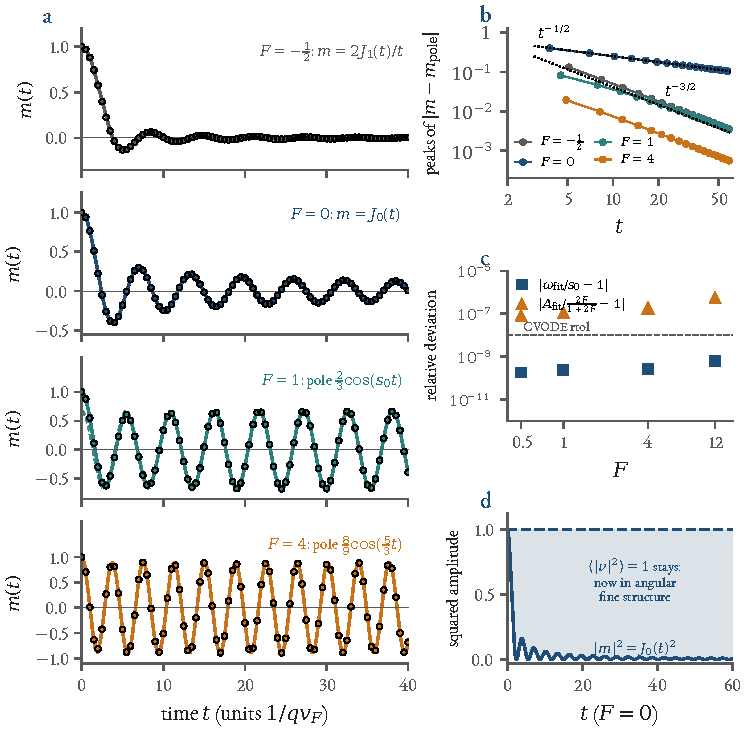
\includegraphics[width=\linewidth]{figures/ch08_timedomain.pdf}
\caption[CVODE against the closed forms of the kinetic equation]{\textbf{CVODE against the closed forms.} Units $v_Fq=1$, BDF, $N=64$, relative tolerance $10^{-8}$.
\textbf{a}, the density amplitude $m(t)$ after a released density wave, for $F=-\frac12$ (exactly $2J_1(t)/t$), $F=0$ ($J_0(t)$), $F=1$ and $F=4$ (the sum \eqref{ch08:eq-uniform} of an undamped line, dashed, and a band that dephases); open circles, CVODE every $0.5$ time units; lines, closed forms.
\textbf{b}, peaks of the part of $m$ that is not the pole: the band's contribution decays algebraically, as $t^{-1/2}$ at $F=0$ and $t^{-3/2}$ otherwise.
\textbf{c}, deviation of the fitted late-time frequency from the Lean root $s_0$ (blue) and of the fitted amplitude from $2F/(1+2F)$ (orange), after the exactly known band part has been subtracted.
\textbf{d}, $F=0$: the squared density amplitude (solid) against the squared norm of the Fermi-circle distortion (dashed); the shading is the part of the distortion no longer visible in the density.
Script: \texttt{figures/ch08\_timedomain.py}.}\label{ch08:fig-timedomain}
\end{figure}

\Cref{ch08:fig-timedomain}a is that formula made visible, and \cref{ch08:tab-solver} gives the numbers.
CVODE agrees with the closed forms at every $F$ tried: the largest deviation over $0\le t\le60$ is $\ceightV{errU_m0p5}$ at $F=-\frac12$ and $\ceightV{errU_0}$ at $F=0$, and grows to $\ceightV{errU_12}$ at $F=12$, where the solution oscillates fastest and more steps accumulate more error; for the kick the deviations of $-\operatorname{Im}m/2$ from the sine transform are $\ceightV{errK_m0p5}$ and $\ceightV{errK_12}$.

The sharpest test against Lean is the pole.
Subtract the exactly known band part of \eqref{ch08:eq-uniform} from the CVODE signal; what remains must be one undamped cosine.
A least-squares fit of $A\cos(\omega t+\varphi)$ over $0\le t\le60$ gives, at $F=4$, $\omega=\ceightV{omegaFit4}$ against the Lean root $s_0=5/3=1.666666667$ and $A=\ceightV{ampFit4}$ against $2F/(1+2F)=8/9$; at $F=\frac12$, $\omega=\ceightV{omegaFit05}$ against $s_0=\ceightV{sZeroHalf}$.
Over $F=\frac12,1,4,12$ the frequency agrees with $s_0$ to a relative $\ceightV{fitW_0p5}$ to $\ceightV{fitW_12}$ and the amplitude with $2F/(1+2F)$ to $\ceightV{fitA_0p5}$ to $\ceightV{fitA_12}$ (\cref{ch08:fig-timedomain}c).
The time integration of the kinetic equation lands on the number that Lean proved to exist, ten digits deep.

\begin{table}[tp]
\centering\small
\caption{\textbf{CVODE (BDF, $N=64$, relative tolerance $10^{-8}$, absolute $10^{-10}$) on the kinetic equation, $0\le t\le60$, against the closed forms.} ``Released'': $\nu\equiv1$; ``kick'': $\nu=\cos\theta$ (not run at $F=0$). Energy drift: $\max_t|E(t)/E(0)-1|$ for the conserved form \eqref{ch08:eq-energy}. Steps for the released runs.}\label{ch08:tab-solver}
\begin{tabular}{@{}r@{\quad}c@{\quad}c@{\quad}c@{\quad}r@{}}
\toprule
$F$ & max error, released & max error, kick & energy drift & steps\\
\midrule
$-\tfrac12$ & \ceightV{errU_m0p5} & \ceightV{errK_m0p5} & \ceightV{edrift_m0p5} & \ceightV{stepsU_m0p5}\\
$0$ & \ceightV{errU_0} & --- & \ceightV{edrift_0} & \ceightV{stepsU_0}\\
$\tfrac12$ & \ceightV{errU_0p5} & \ceightV{errK_0p5} & \ceightV{edrift_0p5} & \ceightV{stepsU_0p5}\\
$1$ & \ceightV{errU_1} & \ceightV{errK_1} & \ceightV{edrift_1} & \ceightV{stepsU_1}\\
$4$ & \ceightV{errU_4} & \ceightV{errK_4} & \ceightV{edrift_4} & \ceightV{stepsU_4}\\
$12$ & \ceightV{errU_12} & \ceightV{errK_12} & \ceightV{edrift_12} & \ceightV{stepsU_12}\\
\bottomrule
\end{tabular}
\end{table}

Two choices about the solver were not free, and a reader reproducing this should know them.
\emph{BDF, not Adams.}
At $F=0$, $N=64$, output every $0.1$, the BDF option reproduces $J_0$ to $\ceightV{tol_bdf_06}$, $\ceightV{tol_bdf_08}$ and $\ceightV{tol_bdf_10}$ at relative tolerances $10^{-6}$, $10^{-8}$, $10^{-10}$; the Adams option of the same crate gives $\ceightV{tol_adams_06}$, $\ceightV{tol_adams_08}$ and $\ceightV{tol_adams_10}$, the first two of the order of the signal itself or larger.
The defect is intermittent.
With only $N=4$ nodes at tolerance $10^{-8}$, Adams is accurate ($\ceightV{sweepAdamsGoodMin}$ to $\ceightV{sweepAdamsGoodMax}$) when the solution is requested every $0.01$, $1$, $5$, $10$, $20$ or $60$ time units, and wrong ($\ceightV{sweepAdamsBad}$; $\ceightV{sweepAdamsBadFD}$ with the Jacobian differenced by CVODE) when it is requested every $0.1$, while BDF stays between $\ceightV{sweepBdfMin}$ and $\ceightV{sweepBdfMax}$ for all seven spacings.
We did not look for the cause; the chapter's runs use BDF.
\emph{The crate, not the installed Python module.}
The module \texttt{rusty\_sundials} in the book's virtual environment (file dated \ceightV{modStaleDate}, the day before the repository's tight-tolerance fix) fails on this system at tolerances $10^{-8}$ and $10^{-10}$ (``too many error test failures at one step''), and its Adams option converges only as the square root of the tolerance, the signature of a first-order method ($\ceightV{mod_stale_adams_06}$, $\ceightV{mod_stale_adams_08}$, $\ceightV{mod_stale_adams_10}$ for $N=32$ to $t=0.5$); a build of commit \texttt{\ceightV{modFreshCommit}} passes the same test with either method (errors $\ceightV{mod_fresh_bdf_06}$ to $\ceightV{mod_fresh_bdf_10}$ for BDF, $\ceightV{mod_fresh_adams_06}$ to $\ceightV{mod_fresh_adams_10}$ for Adams).
Everything in this chapter was computed with the Rust crates directly, at that commit.
Last, $N=96$ instead of $64$ at $F=4$ changes the result by $\ceightV{nNinetySix}$, within tolerance, with $\ceightV{stepsN96}$ steps against $\ceightV{stepsN64}$.

%% ====================================================================================================================
\section{Landau damping is dephasing}\label{ch08:sec-dephasing}

At $F=0$, \cref{ch08:fig-timedomain}a shows a density that dies out, $m=J_0(t)\to0$, in a system without any dissipation.
Where did it go?
The equation \eqref{ch08:eq-kinetic} conserves the quadratic form
\begin{equation}\label{ch08:eq-energy}
E=\ceightavg{|\nu|^2}+F\,|\ceightavg{\nu}|^2 ,\qquad \frac{\dd E}{\dd t}=0 .
\end{equation}
At $F=0$ this is the squared norm of the Fermi-circle distortion, and $\ceightavg{|\nu|^2}=1$ for all time (the solver keeps it to $\ceightV{normDrift}$ up to $t=60$) while $|m|^2=J_0(t)^2$ has fallen to $\ceightV{mSqEnd}$ (\cref{ch08:fig-timedomain}d).
The amplitude of the distortion is intact; it has moved from the angular average, which the density sees, into angular structure of ever finer scale.
Landau damping is dephasing, not dissipation: each direction oscillates at its own frequency $v_Fq\cos\theta$, and the average over directions loses coherence.

\Cref{ch08:fig-fermisurface} shows it directly.
It plots the Fermi circle itself, $r=1+\epsilon\operatorname{Re}\nu(\theta,t)$, at the place where the density wave has its maximum, for $F=0$ and $F=4$ (the profile on a fine angular grid is reconstructed from the CVODE solution by the exact Duhamel formula $\nu=\ee^{-\ii ct}\bigl[\nu_0-\ii Fc\int_0^t\ee^{\ii ct'}m(t')\,\dd t'\bigr]$, $c=\cos\theta$, and agrees with the solver's node values to $\ceightV{reconF0}$ and $\ceightV{reconF4}$).
At $F=0$ the ripples multiply in proportion to $t$, because the phase $t\cos\theta$ changes with $\theta$ at the rate $t\sin\theta$; near $\theta=0$ and $\pi$ it does not change, to first order.
Those are the quasi-particles that move along the wave vector at the speed of the wave: they do not dephase, and they are the resonance of \cref{ch08:sec-model}.
At $F=4$ the same filaments are present and, on top of them, a large smooth distortion of the circle, flattened at $\theta=0,\pi$ and bulging at $\pm\pi/2$ at one moment and the reverse half a period later: zero sound, a collective mode of the whole circle, with a maximum $|\nu|$ of $\ceightV{nuMaxFour12}$ at $t=12$.

\begin{figure}[tp]
\centering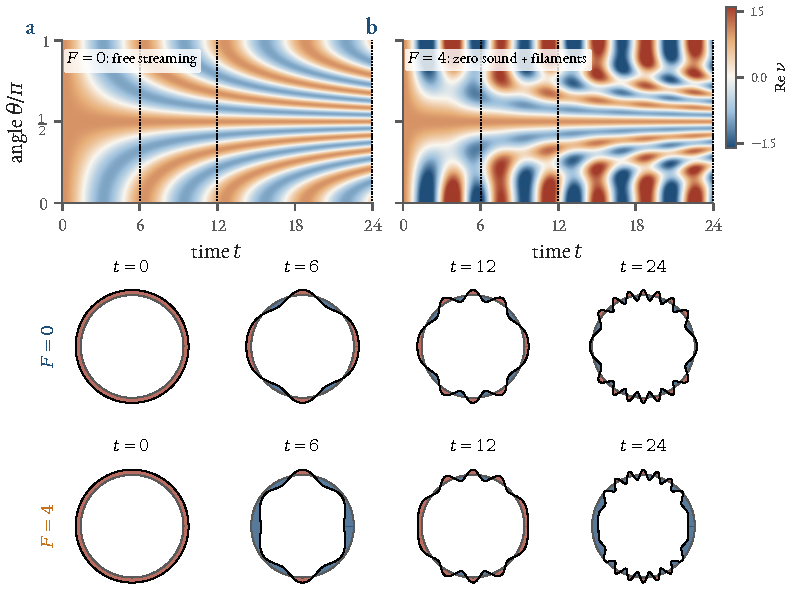
\includegraphics[width=\linewidth]{figures/ch08_fermisurface.pdf}
\caption[The Fermi circle as the dynamical variable]{\textbf{The Fermi circle as the dynamical variable.}
Top: $\operatorname{Re}\nu(\theta,t)$ after a released density wave, $F=0$ (free streaming: a fan of stripes, pitch shrinking as $1/t$ except at $\theta=0,\pi$) and $F=4$ (zero sound at $s_0=5/3$: large smooth lobes near $\theta=0$ and $\pi$ on top of the same fan); the colour scale saturates at $\pm1.6$.
Below: the circle $r=1+\epsilon\operatorname{Re}\nu$, $\epsilon=\ceightV{epsFS}$ (deformation magnified, the same $\epsilon$ in every panel; red outward, blue inward) at $t=0,6,12,24$; the wave vector points to the right.
At $F=0$ the circle keeps $\ceightavg{|\nu|^2}=1$ while the density average decays: the amplitude has moved into the ripples.
Script: \texttt{figures/ch08\_fermisurface.py}.}\label{ch08:fig-fermisurface}
\end{figure}

The decay law of what is left in the density comes from the edge of the continuum.
The part of $m$ that is not the pole is the cosine transform of a spectral density that vanishes like $(1-y)^{1/2}$ at the edge $y=1$ for every $F\ne0$, and diverges like $(1-y)^{-1/2}$ at $F=0$, where the denominator in \eqref{ch08:eq-uniform} vanishes at $y=1$; the transforms decay as $t^{-3/2}$ and $t^{-1/2}$.
The solver reproduces both: the fitted slopes of the envelope of the non-pole part over $10\le t\le60$ are $\ceightV{expo_0}$ at $F=0$ and $\ceightV{expo_m0p5}$ at $F=-\frac12$ (\cref{ch08:fig-timedomain}b), and $\ceightV{expo_4}$ at $F=4$; at $F=1$, where the asymptotics sets in later, it is $\ceightV{expo_1}$ in this window.

The library holds the field-free core of this picture.
The module \texttt{PhaseMixing} proves, with no regularity assumed, that the $k$-th density mode of free transport $\ee^{\ii k(x-vt)}g(v)$ tends to zero (\Lthm{PhaseMixing}{phase_mixing}, an application of the Riemann--Lebesgue lemma), and that for the unit Maxwellian it is exactly $\ee^{-k^2t^2/2}$ (\Lthm{PhaseMixing}{maxwellian_mode}, quoted in \cref{ch08:sec-vlasov}); for the circle the analogue is $J_0$, which is not in the library.
That module is subsumed by Bedrossian's Lean formalisation of the nonlinear Mouhot--Villani theorem \cite{MouhotVillani2011,Bedrossian2026} and claims nothing beyond the linear statement.

Finally, \eqref{ch08:eq-energy} is the energy of the Pomeranchuk bound.
Because $|\ceightavg\nu|^2\le\ceightavg{|\nu|^2}$, one has $E\ge\min(1,1+F)\ceightavg{|\nu|^2}$: for $F>-1$ the form is positive definite and every solution of the single-wave model stays bounded.
Below the bound it is indefinite and the model has a growing solution: with $s=\ii y$, \eqref{ch08:eq-disp} reads $1+F\bigl(1-y/\sqrt{1+y^2}\bigr)=0$, solved by $y=r/\sqrt{1-r^2}$, $r=1-1/|F|$, once $F<-1$; at $F=-2$, $y=1/\sqrt3=\ceightV{growthPred}$.
CVODE at $F=-2$ grows as $\ee^{yt}$ with the fitted rate $\ceightV{growthFit}$ over $10\le t\le14$, $E$ conserved to $\ceightV{growthEdrift}$.
This is a simulation of an elementary instability, not a theorem: the library contains no stability theorem for the Landau equation (\cref{ch08:honest}, item 3).

%% ====================================================================================================================
\section{A plasma cousin, and the property that decides}\label{ch08:sec-vlasov}

Equation \eqref{ch08:eq-kinetic} resembles the Vlasov equation of a plasma, and the rusty-SUNDIALS repository has a solver for one: the crate \texttt{qf-vlasov1d}, one space and one velocity dimension, electrons on a neutralising background (units of the plasma frequency),
\begin{equation}\label{ch08:eq-vlasov}
\partial_tf+v\,\partial_xf-E\,\partial_vf=0,\qquad \partial_xE=1-\!\int\! f\,\dd v .
\end{equation}
It advances $x$ by an exact Fourier shift and $v$ by a cubic semi-Lagrangian step (a natural spline, a documented departure from its Python original), in Strang splitting, on $32\times512$ cells with $|v|\le6$ and time step $0.1$.
Two backgrounds $f_0(v)$ of equal density are used: a Maxwellian, and a degenerate Fermi--Dirac profile $f_0\propto[1+\ee^{(|v|-v_0)/w}]^{-1}$ with $v_0=1$, $w=0.1$, a sea with two smeared edges that is the one-dimensional Fermi surface.
The Maxwellian is perturbed in density, $f_0(1+a\cos kx)$; the degenerate sea by displacing its edges, $v_0\to v_0(1+a\cos kx)$, so that the perturbation lives where a Fermi gas can have one.

\begin{rustbox}{qf-vlasov1d on two backgrounds}
From the driver \texttt{book/rust/ch08\_vlasov}: the two backgrounds on the velocity grid, and the evolution (excerpt).
\begin{lstlisting}[style=rust]
Bg::Maxwell => maxwellian(v, 0.0),
Bg::Fermi { v0, w } => 1.0 / (1.0 + ((v.abs() - v0) / w).exp()),
...
let g = Grid::new(2.0 * PI / k, 32, nv, 6.0);
let f0 = initial(&g, bg, a);
run(f0, &g, dt, t_end, observe, field_on,
    Vec::<(f64, fn(&[f64]) -> Vec<f64>)>::new());
\end{lstlisting}
\end{rustbox}

The linear theory is a dispersion relation of the type \eqref{ch08:eq-disp}: $1-k^{-2}\int f_0'(v)\,(v-\omega/k)^{-1}\dd v=0$ along Landau's contour.
For the Maxwellian it is the textbook relation with the plasma dispersion function; at $k=\tfrac12$ it has the root $\omega=\ceightV{vmCertRe}-\ceightV{vmCertIm}\,\ii$ (our mpmath calculation), which agrees with the programme's certified root of its earlier kinetic benchmark ($\ceightV{vmProgRe}-\ceightV{vmProgIm}\,\ii$ to the digits printed) to $\ceightV{vmCertDiff}$.
\Cref{ch08:fig-vlasov} shows both runs.
With the Maxwellian the density perturbation is sheared into filaments of ever finer velocity structure, pitch $2\pi/(kt)$, and the field decays as $\ee^{\gamma t}$ with $\gamma=-\ceightV{vmG_0p5}$.
With the degenerate sea the same density wave rides on the two Fermi edges and does not decay.
Least-squares fits of the solver's signed density mode over $5\le t\le40$ (amplitude, rate, frequency and phase free) give \cref{ch08:tab-vlasov}: for the Maxwellian the rates agree with the roots within $\ceightV{vmRelG_0p3}$ at $k=0.3$, where the mode has lost only $\ceightV{vmLost03}$ of its amplitude by $t=40$, and to better than $\ceightV{vmRelG_0p5}$ from $k=\tfrac12$ up, with frequencies within $\ceightV{vmRelW_0p4}$; going from $n_v=128$ to $256$ to $512$ moves the fitted rates by at most $\ceightV{vmConvMax}$.

\begin{table}[tp]
\centering\small
\caption{\textbf{qf-vlasov1d against linear theory} ($k$ in inverse Debye lengths; $n_v=512$): fits of the signed density mode over $5\le t\le40$ (Maxwellian: the window ends when the mode falls below $3\times10^{-5}$ of its maximum) and the degenerate profile $v_0=1$, $w=0.1$. Degenerate theory: continued root at $k=0.5,\,0.8$, weak-damping formula at $k=0.3$. Rates below about $10^{-4}$ are at the resolution of the fit (residual $\ceightV{vfRes_0p5}$ of the signal at $k=0.5$).}\label{ch08:tab-vlasov}
\begin{tabular}{@{}l@{\quad}c@{\quad}c@{\quad}c@{\quad}c@{\quad}c@{\quad}c@{}}
\toprule
 & $k$ & $\omega_{\rm theory}$ & $\omega_{\rm solver}$ & $|\gamma|_{\rm theory}$ & $|\gamma|_{\rm solver}$ & rel.\ diff.\ $\gamma$\\
\midrule
Maxwellian & 0.3 & \ceightV{vmW_0p3} & \ceightV{vmWs_0p3} & \ceightV{vmG_0p3} & \ceightV{vmGs_0p3} & \ceightV{vmRelG_0p3}\\
 & 0.5 & \ceightV{vmW_0p5} & \ceightV{vmWs_0p5} & \ceightV{vmG_0p5} & \ceightV{vmGs_0p5} & \ceightV{vmRelG_0p5}\\
 & 0.8 & \ceightV{vmW_0p8} & \ceightV{vmWs_0p8} & \ceightV{vmG_0p8} & \ceightV{vmGs_0p8} & \ceightV{vmRelG_0p8}\\
\midrule
degenerate & 0.3 & \ceightV{vfW_0p3} & \ceightV{vfWs_0p3} & \ceightV{vfG_0p3} & \ceightV{vfGs_0p3} & ---\\
 & 0.5 & \ceightV{vfW_0p5} & \ceightV{vfWs_0p5} & \ceightV{vfG_0p5} & \ceightV{vfGs_0p5} & ---\\
 & 0.8 & \ceightV{vfW_0p8} & \ceightV{vfWs_0p8} & \ceightV{vfG_0p8} & \ceightV{vfGs_0p8} & \ceightV{vfRelG_0p8}\\
\bottomrule
\end{tabular}
\end{table}

\begin{figure}[tp]
\centering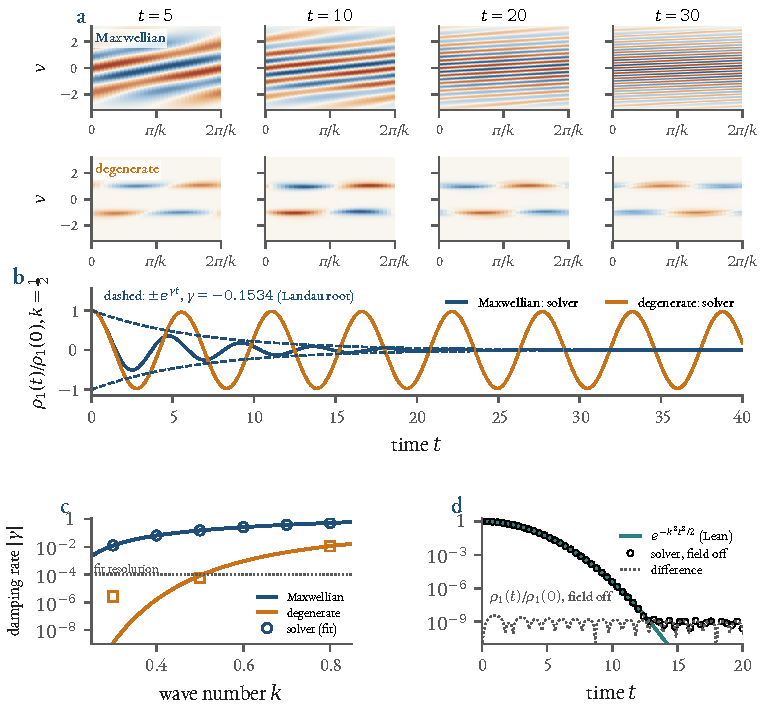
\includegraphics[width=\linewidth]{figures/ch08_vlasov.pdf}
\caption[Vlasov--Poisson: the same density wave on two backgrounds]{\textbf{Vlasov--Poisson (\texttt{qf-vlasov1d}): the same density wave on two backgrounds.}
\textbf{a}, the perturbation $f(x,v,t)-\bar f_0(v)$ at $k=\frac12$, $a=0.05$, $t=5,10,20,30$ (colour scale per row): for the Maxwellian (top) filaments of velocity pitch $2\pi/kt$; for the degenerate sea (bottom) a pair of edge waves.
\textbf{b}, the density mode $\rho_1(t)/\rho_1(0)$ at $k=\frac12$, $a=0.01$: damped (blue; dashed, the envelope $\pm\ee^{\gamma t}$ with the Landau root) and undamped (orange).
\textbf{c}, damping rate against $k$: linear theory (lines) and solver fits (symbols); the degenerate curve is the weak-damping formula, and solver rates below about $10^{-4}$ are at the resolution of the fit.
\textbf{d}, the field-off control: the density mode of free streaming (circles) against $\ee^{-k^2t^2/2}$ (line; Lean: \Lthm{PhaseMixing}{maxwellian_mode}); dotted, the difference, at the floor set by cutting the Maxwellian at $|v|=6$.
Script: \texttt{figures/ch08\_vlasov.py}.}\label{ch08:fig-vlasov}
\end{figure}

The degenerate background tells the other half.
Its roots are $\omega=\ceightV{vfW_0p3}$, $\ceightV{vfW_0p5}$, $\ceightV{vfW_0p8}$ at $k=0.3,\,0.5,\,0.8$, with damping rates $\ceightV{vfG_0p3}$, $\ceightV{vfG_0p5}$ and $\ceightV{vfG_0p8}$: exponentially small at small $k$ because the phase velocity $\omega/k$ lies several widths $w$ beyond the edge $v_0$, where the resonant fraction is $\sim\ee^{-(\omega/k-v_0)/w}$.
The solver's frequencies are $\ceightV{vfWs_0p3}$, $\ceightV{vfWs_0p5}$, $\ceightV{vfWs_0p8}$, and its damping rate at $k=0.8$, large enough to measure, is $\ceightV{vfGs_0p8}$ against $\ceightV{vfG_0p8}$.
At $k=0.3$ and $0.5$ the true rates are below the resolution of the fit; what the solver supports is $|\gamma|<10^{-4}$, three orders of magnitude below the Maxwellian $\ceightV{vmG_0p5}$ at $k=\tfrac12$.
The field-off control is the Lean statement in numbers: with the field switched off, the density mode of the Maxwellian run is $\ee^{-k^2t^2/2}$ to $\ceightV{fsMax}$ over $0\le t\le40$, down to a floor of $\ceightV{fsFloor}$ set by the cut at $|v|=6$, and the free-streaming recurrence, an artefact of any velocity grid at $t=2\pi/(k\,\Delta v)=\ceightV{fsRecur}$, is far outside the window.

\begin{leanbox}[unbreakable]{PhaseMixing}
\begin{lstlisting}[style=lean]
theorem maxwellian_mode (k t : ℝ) :
    ∫ v : ℝ, cexp (-((k * v * t : ℝ) : ℂ) * I) *
        ((rexp (-v ^ 2 / 2) / √(2 * π) : ℝ) : ℂ)
      = cexp (-((k * t) ^ 2 / 2 : ℝ))
\end{lstlisting}
\end{leanbox}

\begin{keybox}[An analogy is not a result]
The finding is ``a collective mode of a collisionless kinetic equation is damped by phase mixing''.
The tempting transfer: the plasma shows Landau damping, so Fermi-liquid zero sound is Landau damped.
What the finding depends on is not the form of the equation, which the two systems share, but the \emph{support} of the velocity distribution relative to the phase velocity of the wave.
A Maxwellian has unbounded support, so some particles always move at the phase velocity and the mode is damped at a rate fixed by $f_0'(\omega/k)$; a degenerate gas has bounded support, and a wave faster than the edge has no resonant particles.
The degenerate run shows precisely this, and a Fermi circle has the property: $s>1$ in \eqref{ch08:eq-disp} is its statement.
What does \emph{not} transfer is any number: the plasma's interaction is a long-range force of strength $1/k^2$ where the Fermi liquid has the contact parameter $F$, the roots solve different equations, and the rate $\ceightV{vmG_0p5}$ is a fact about electrons on a Maxwellian background and nothing about helium.
\end{keybox}

%% ====================================================================================================================
\section{Beyond Landau: the window at twice the Fermi momentum}\label{ch08:sec-window}

\begin{figure}[tp]
\centering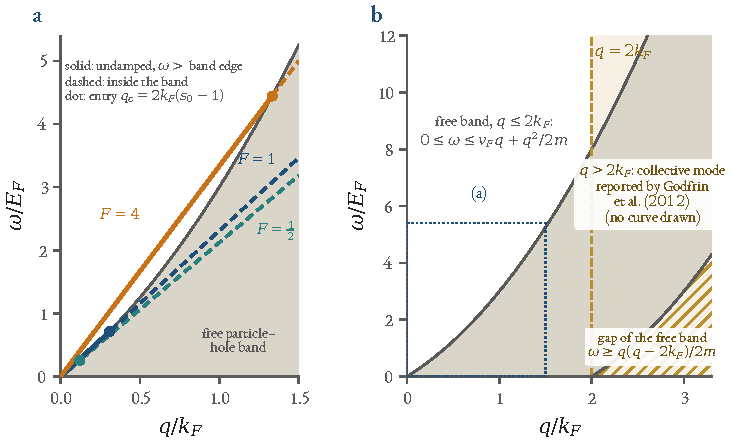
\includegraphics[width=\linewidth]{figures/ch08_window.pdf}
\caption[The $(q,\omega)$ plane in free-gas units]{\textbf{The $(q,\omega)$ plane, in free-gas units} ($q/k_F$, $\omega/E_F$ with $E_F=\hbar^2k_F^2/2m$, so that $v_Fq=2(q/k_F)E_F$).
\textbf{a}, the Landau line $\omega=s_0v_Fq$ for $F=\frac12,1,4$ against the upper edge $v_Fq+\hbar q^2/2m$ of the free particle--hole band (grey): solid where the line is above the edge (undamped), dashed once inside (damped), dot at the entry $q_c=2k_F(s_0-1)$.
\textbf{b}, the whole free band up to $3.3\,k_F$: its lower edge is $0$ for $q\le2k_F$ and $\hbar q(q-2k_F)/2m$ for $q>2k_F$ (hatched, the gap; Lean: \Lthm{ZeroSound2D}{ph_gap}); gold, the momentum transfers $q>2k_F$ at which Godfrin \emph{et al.}\ report the reappearing collective mode.
No curve is drawn there.
Script: \texttt{figures/ch08\_window.py}.}\label{ch08:fig-window}
\end{figure}

What does the model say about the third regime of \cref{ch08:sec-measure}?
Nothing, and it is worth seeing why.
The model's collective mode is the straight line $\omega=s_0v_Fq$, derived for $q\ll k_F$ with a single parameter $F$ and no scale at which a minimum could form.
Against the free-gas band of \cref{ch08:fig-window}a the line enters the edge $v_Fq+\hbar q^2/2m$ at $q_c=2k_F(s_0-1)$, which is $\ceightV{qc_0p5}\,k_F$ at $F=\frac12$, $\ceightV{qc_1}\,k_F$ at $F=1$, $\ceightV{qc_4}\,k_F$ at $F=4$ and $\ceightV{qc_12}\,k_F$ at $F=12$ (for $F\ge3+2\sqrt3=\ceightV{Fstar}$ it stays above the edge up to $q=2k_F$); beyond $q_c$ the model's answer is a broadened line.
That is the second regime of the abstracts, in outline: the zero-sound mode enters the band and is damped.
It is not a quantitative claim about the film, whose $F$, effective mass and $k_F$ are not known here; and for the larger values of $F$ the entry point is at $q_c\gtrsim k_F$, outside the range $q\ll k_F$ for which the straight line was derived.

The one exact statement about the third regime that survives in this framework is kinematic and holds for the free gas: the band has a lower edge, and the edge lifts off $\omega=0$ at $q=2k_F$.

\begin{leanbox}{Ch08\_ZeroSound2D (new in this book)}
\begin{lstlisting}[style=lean]
theorem ph_gap {E : Type*} [NormedAddCommGroup E]
    [InnerProductSpace ℝ E] {m kF : ℝ} (hm : 0 < m)
    (hkF : 0 ≤ kF) (k q : E) (hk : ‖k‖ ≤ kF)
    (hq : 2 * kF < ‖q‖) :
    0 < ‖q‖ * (‖q‖ - 2 * kF) / (2 * m) ∧
      ‖q‖ * (‖q‖ - 2 * kF) / (2 * m)
        ≤ (‖k + q‖ ^ 2 - ‖k‖ ^ 2) / (2 * m)
\end{lstlisting}
\end{leanbox}

A hole of momentum $k$ inside the Fermi sphere ($\|k\|\le k_F$) and a particle of momentum $k+q$ cost the energy $(\|k+q\|^2-\|k\|^2)/2m$ (with $\hbar=1$).
The gap theorem says that for $q>2k_F$ every such pair costs at least $q(q-2k_F)/2m>0$.
It rests on \Lthm{ZeroSound2D}{ph_energy_window}, which puts the cost between $(q^2-2k_Fq)/2m$ and $(q^2+2k_Fq)/2m$ in \emph{any} real inner-product space, hence for the film and for the bulk liquid alike; the proof is the Cauchy--Schwarz inequality $|\langle k,q\rangle|\le k_Fq$ and nothing else.
And \Lthm{ZeroSound2D}{ph_edge_attained} says the lower bound is reached, by the hole $k=-(k_F/\|q\|)\,q$ on the Fermi surface, whose partner $k+q$ lies outside it as soon as $\|q\|\ge2k_F$.
For $q<2k_F$ the lower edge is zero, because the bound is negative and a pair at the Fermi surface can cost arbitrarily little.

This is the mathematics of the number $2k_F$ in the 2012 abstract: the collective mode is said to reappear at momentum transfers larger than twice the Fermi momentum, and $2k_F$ is where the free band opens a window below itself.
The coincidence is noted; it is not claimed as the explanation.
The abstracts say that the reappearing excitation lies ``beyond the particle-hole band'', with a dispersion ``quite similar to that of superfluid $^4$He'', and that a dynamic many-body theory interprets the spectra.
Whether the observed mode sits in the free band's window, how the interaction pushes it, and why it has a minimum are exactly what a theory of pair fluctuations beyond the Landau parameter must answer, and what this book's tools do not reach; the Godfrin--Krotscheck survey \cite{GodfrinKrotscheck2022} is the place to read how the question is treated.
In the helium-4 chapters the roton is a feature of a measured curve (\cref{ch05}); here it is a feature that a measurement found in a system where the standard theory did not expect it.

%% ====================================================================================================================
\section{What is established, and what is not}\label{ch08:honest}

\begin{honestbox}
\textbf{Proved (Lean, standard axioms only).} The library: \Lthm{ZeroSound}{zero_sound_2d_iff} and \Lthm{ZeroSound}{zero_sound_iff} (an undamped zero-sound root $s>1$ exists iff $F>0$; 2D with the explicit root, 3D by pinning and the intermediate value theorem) and \Lthm{PhaseMixing}{maxwellian_mode}.
New in this book, in \texttt{book/lean/Ch08\_ZeroSound2D.lean} (namespace \texttt{QuantumFluids.ZeroSound2D}): uniqueness of the 2D root, the derivative of $\Omega_{2\mathrm D}$, the residue weight and its share of the first moment, and the free-gas particle--hole window.
The file compiles with the pinned Lean 4 and Mathlib with no \texttt{sorry}; \texttt{\#print axioms} reports \ceightV{leanAxioms} for each of its nine theorems.
These are statements about mathematics; that a helium film obeys them is physics.\par\vspace{3pt}
\textbf{Derived and checked numerically, not in Lean.} The structure factor \eqref{ch08:eq-S}; the residue as the strength of a $\delta$-function; the $f$-sum rule \eqref{ch08:eq-fsum} (the quadrature closes it to $\ceightV{sumDev}$); the exact solutions $J_0$ and $2J_1(t)/t$ and the formula \eqref{ch08:eq-uniform}; the conserved form \eqref{ch08:eq-energy}.\par\vspace{3pt}
\textbf{Simulated.} CVODE (BDF) on the kinetic equation (errors $\ceightV{errU_m0p5}$ to $\ceightV{errU_12}$ against the closed forms) and on the root continuation; \texttt{qf-vlasov1d}.\par\vspace{3pt}
\textbf{Measured, by others.} Everything about helium, by Godfrin and his collaborators \cite{Godfrin2010,Godfrin2012}, quoted from their abstracts.
This book has no spectra and no film parameters; every number here is a function of the free $F$.\par\vspace{3pt}
\textbf{Only an analogy.} Plasma against Fermi liquid.
What they share (free streaming plus a mean field, dephasing) is real, and the degenerate run confirms the property that decides whether a mode is damped (bounded support); the plasma's numbers say nothing about helium.\par\vspace{3pt}
\textbf{Not claimed, and not possible here.} The roton; any finite-$q$ or finite-temperature statement; $F_1^s$ and the effective mass; collisions and the crossover from zero to first sound; a comparison with the film.
Past the line the model draws, the chapter says only what is free-gas kinematics.\par\vspace{3pt}
\textbf{What failed or was withdrawn.}
(1) The installed Python module of CVODE failed on this problem, and the Adams option of the crate gave wrong answers at one output spacing (\cref{ch08:sec-cvode}); reported, not investigated.
(2) A first estimate of the Vlasov damping rates from the spacing of field maxima returned a positive rate for the weakly damped degenerate run ($+\ceightV{peakFitFermi05}$ at $k=0.5$); it was replaced by least-squares fits, and rates below about $10^{-4}$ are not claimed.
(3) The programme's attempt to formalise a Pomeranchuk--Penrose stability theorem for the 2D Landau equation was stopped at its literature gate (CLAIM-030); the library has none.
(4) The programme's two searches for the 2D Landau parameters of the film found no open table (CLAIM-030, CLAIM-031); the ledger names the 2010 paper as a likely source, and only its abstract, which gives no parameter, was read for this chapter.
\end{honestbox}

%% ====================================================================================================================
\section*{Exercises}

\paragraph{Exercise 1.}
Show that squaring $1+F\,\Omega_{2\mathrm D}(s)=0$ gives $s^2(1+2F)=(1+F)^2$, and that the positive root solves the unsquared equation exactly when $F>0$.
Expand $s_0$ for small $F$ to order $F^3$ and verify $s_0^2=\frac F2+\frac34+\frac1{4(1+2F)}$.
\emph{Hint.} $(1+F)^2-F^2=1+2F$; the unsquared equation needs $Fs/(1+F)>0$, which is where the sign of $F$ enters. Answer: $s_0-1=F^2/2-F^3+O(F^4)$.

\paragraph{Exercise 2.}
Derive \eqref{ch08:eq-W} from $\Omega'(s)=(s^2-1)^{-3/2}$ and \eqref{ch08:eq-root}, then \eqref{ch08:eq-frac}.
For which $F$ does the zero-sound line carry $90\,\%$ of the first moment?
Show also that \eqref{ch08:eq-fsum} follows from $G(s)\simeq-1/(2s^2)$ at large $|s|$.
\emph{Hint.} $s_0W=F(1+F)/(1+2F)^2$ and $4F(1+F)=(1+2F)^2-1$; the first answer is $(1+2F)^2=10$, i.e.\ $F=(\sqrt{10}-1)/2=\ceightV{Fninety}$.

\paragraph{Exercise 3.}
Prove that $E=\ceightavg{|\nu|^2}+F|\ceightavg\nu|^2$ is constant along solutions of \eqref{ch08:eq-kinetic} for a single wave vector, and that for $F>-1$ every solution is bounded.
Then find the growth rate for $F<-1$ and compare it with the CVODE run at $F=-2$ of \cref{ch08:sec-dephasing}.
\emph{Hint.} Differentiate both terms: only the cross terms $\pm2F\operatorname{Re}[\ii\,m^*\ceightavg{\cos\theta\,\nu}]$ survive, and they cancel; $\ceightavg{\cos\theta}=0$ removes the $Fm$ term from $\dot m$. For the rate put $s=\ii y$ and use $\ceightavg{(\cos^2\theta+y^2)^{-1}}=1/(y\sqrt{1+y^2})$.

%% ====================================================================================================================
\section*{Notes and further reading}

Landau's theory of the Fermi liquid is in his 1957 paper \cite{Landau1957}; its textbook presentation, with the kinetic equation, the Landau parameters and zero sound, is Baym and Pethick \cite{BaymPethick1991}.
Zero sound was observed in liquid $^3$He by Abel, Anderson and Wheatley in 1966 \cite{AbelAndersonWheatley1966}.
The measurements this chapter is organised around are \cite{Godfrin2010,Godfrin2012}, and the Godfrin--Krotscheck survey of excitation spectra of quantum fluids \cite{GodfrinKrotscheck2022} puts them in context.
Landau damping as a theorem (nonlinear, Vlasov--Poisson) is due to Mouhot and Villani \cite{MouhotVillani2011}, its Lean 4 formalisation to Bedrossian \cite{Bedrossian2026}; the library module used here, \texttt{PhaseMixing}, is only the linear field-free core \cite{Callens2026lib}.
The solver is the CVODE of SUNDIALS \cite{Hindmarsh2005} as ported to Rust in rusty-SUNDIALS (commit \texttt{5db8041}); the proof assistant is Lean 4 with Mathlib \cite{deMoura2021,Mathlib2020}.
\renewcommand{\topfraction}{0.7}\renewcommand{\textfraction}{0.2}\renewcommand{\floatpagefraction}{0.5}\setcounter{topnumber}{2}
